\documentclass[12pt,aspectratio=43,hyperref={unicode}]{beamer}

% \documentclass[aspectratio=43]{beamer}
% \documentclass[aspectratio=1610]{beamer}
% \documentclass[aspectratio=169]{beamer}

%\usepackage{lmodern}

% подключаем кириллицу
% \usepackage[T2A]{fontenc}
% \usepackage[utf8]{inputenc}
% \usepackage[ukrainian]{babel}

\usepackage{scrextend}
\usepackage[no-math]{fontspec} % костыль
\usepackage{mathspec}
\usepackage{xunicode,xltxtra} % не мешает вроде
\usepackage{mathptmx}
\usepackage{multicol}

% ПОЛИГЛОССИЯ
\usepackage{polyglossia} % на замену babel
\setmainlanguage{ukrainian}
\defaultfontfeatures{Mapping=tex-text} % чтобы работали "---" и прочее
\setotherlanguages{english, russian}
\newfontfamily\cyrillicfont[Script=Cyrillic]{Arial}
\newfontfamily\cyrillicfonttt[Script=Cyrillic]{Arial}

% СТАВИМ ШРИФТЫ
\setsansfont{Arial}
\setmainfont[Scale=1]{Arial} % .976
\setmathfont(Digits,Latin,Greek)[Scale=1, Numbers={Lining,Proportional}]{Arial}
\setmonofont{Arial}
%\linespread{1.5} % 1.464

%выключаем переносы и делаем выравнивание текста Word-like
\tolerance=1
\emergencystretch=\maxdimen
\hyphenpenalty=10000
\hbadness=10000

%\usepackage{ragged2e}
%\renewcommand{\raggedright}{\leftskip=0pt \rightskip=0pt plus 0cm}
% делаем чтобы запятые в формулах были тоже таймс нью роман
%\usepackage[output-decimal-marker=\textrm{,}]{siunitx}
%\renewcommand\materialfont{\sffamily\fontsize{7pt}{\baselineskip}\selectfont}

%\setbeamertemplate{caption}{\insertcaption}
%\setbeamertemplate{caption label}{}
%\setbeamertemplate{caption label separator}{}
% тема оформления
\usetheme{Luebeck}
%\usefonttheme{cmss} % using non standard fonts for beamer


\graphicspath{{./figures/}}

% отключить клавиши навигации
\setbeamertemplate{navigation symbols}{}
\setbeamertemplate{footline}[frame number]
\setbeamerfont{footline}{size=\fontsize{12}{12}\selectfont}
%\setbeamertemplate{caption}[numbered]
\setbeamertemplate{caption}{\raggedright\insertcaption\par}

\setbeamertemplate{headline}{}

\makeatletter
\def\beamer@framenotesbegin{% at beginning of slide
  \ifnum \value{framenumber}>1
  \frametitle{\small\bf\insertsectionhead}
  \framesubtitle{\small\bf\insertsubsectionhead}
  \else
  \fi
}
\makeatother


\setbeamertemplate{frametitle}{%
  \nointerlineskip
    \begin{beamercolorbox}[sep=0.5ex,wd=\paperwidth,leftskip=1cm,rightskip=0cm]{frametitle}%
      \usebeamerfont{frametitle}\usebeamercolor[fg]{frametitle}\insertframetitle\\
      \usebeamerfont{framesubtitle}\usebeamercolor[fg]{framesubtitle}\insertframesubtitle
    \end{beamercolorbox}%
}


% цветовая схема
% \usecolortheme{seagull}

%\hyphenpenalty=100000 %%% to turn the hyphenation off

\PassOptionsToPackage{demo}{graphicx}

\makeatletter
\let\insertsupervisor\relax
\newcommand\supervisortitle{Керівник}
\mode<all>
{
  \newcommand\supervisor[1]{\def\insertsupervisor{#1}}
  \titlegraphic{}
}
\defbeamertemplate*{title page}{supdefault}[1][]
{
  \vbox{}
  %\vfill
  \begingroup
    \centering
    \begin{beamercolorbox}[sep=4pt,center,#1]{institute}
      \usebeamerfont{institute}\insertinstitute
    \end{beamercolorbox}
    \begin{beamercolorbox}[sep=8pt,center,#1]{title}
      \usebeamerfont{title}\inserttitle\par%
      \ifx\insertsubtitle\@empty\relax%
      \else%
        \vskip0.25em%
        {\usebeamerfont{subtitle}\usebeamercolor[fg]{subtitle}\insertsubtitle\par}%
      \fi%
    \end{beamercolorbox}%
    %\vskip1em\par
    \begin{beamercolorbox}[sep=4pt,center,#1]{author}
      \usebeamerfont{author}
      \begin{flushright}
      \begin{tabular}{rl}
        \textbf{Виконав:}&студент групи ФМ-31\\
        &\insertauthor\\
        \textbf{\supervisortitle:}&\insertsupervisor
      \end{tabular}
      \end{flushright}
    \end{beamercolorbox}

    \begin{beamercolorbox}[sep=4pt,center,#1]{date}
      \usebeamerfont{date}\insertdate
    \end{beamercolorbox}%\vskip0.5em
    {\usebeamercolor[fg]{titlegraphic}\inserttitlegraphic\par}
  \endgroup
  \vfill
}
%\setbeamertemplate{title page}[supdefault][colsep=-4bp,rounded=true,shadow=\beamer@themerounded@shadow]\makeatother

\expandafter\def\expandafter\normalsize\expandafter{%
    \normalsize
    \setlength\abovedisplayskip{0pt}
    \setlength\belowdisplayskip{0pt}
    \setlength\abovedisplayshortskip{0pt}
    \setlength\belowdisplayshortskip{0pt}
}


%\title{Дипломна робота на тему:}
\title{Створення функціональних покриттів на сталі~45 пошаровим електроіскровим легуванням хромом, вольфрамом та графітом}
\author{Богомаз Р.Д.}
\supervisor{к.т.н. Лобачова Г.Г.}
\date{}
%\institute{Інженерно-Фізичний факультет\\Кафедра Фізики Металів}
%\logo{\includegraphics[height=10mm]{logo.jpg}\vspace{900pt}}
    \titlegraphic{\includegraphics[width=2cm,height=2cm]{logo.jpg}}

\begin{document}

% титульный слайд
\begin{frame}[plain]
  \titlepage
\end{frame}

\section{Актуальність}
\begin{frame}

\centering
\includegraphics[width=\textwidth, trim={1.5cm 0cm 1.5cm 1.5cm},clip]{graph.pdf}
% ТРАДИЦІЙНО (ЧЕРВОНИМ) : компактовані аноди

% TODO ЗРОБИТИ МАЛЮнОК АКТУАЛЬНОСТІ

%Для зміцнення та нанесення захисних поверхонь вигідно використовувати електрофізичні методи обробки матеріалів, сутність яких полягає на використанні концентрованих потоків енергії. Одним із таких методів є електроіскрове легування (ЕІЛ) металевих поверхонь. Його основними перевагами є економічність, екологічність та простота відтворення. Також цей метод дає широкий спектр можливих варіантів проведення експерименту в залежності від обраних матеріалів та відповідно отриманих властивостей поверхні.

\end{frame}


\section{Мета роботи} % TODO ПЕРЕРОБИТИ
\begin{frame}

\begin{block}{\textbf{Дослідження}}
\vspace{-0.3cm}
\begin{itemize}
  \item структури,
  \item фазового складу
  \item та властивостей покриттів
\end{itemize}
одержаних пошаровим нанесенням
\begin{itemize}
  \item вольфраму,
  \item хрому
  \item та графіту
\end{itemize}
на поверхню сталі~45 в процесі електроіскрового легування.
\end{block}


\end{frame}

\section{Методика дослідження}
\begin{frame}
  \begin{itemize}
  \item \textbf{\large Мікроструктурний аналіз}\\
  ~
  \item \textbf{\large Гравіметричний аналіз}\\%<3->
  ~
  \item \textbf{\large Рентгеноструктурний аналіз}\\
    ~
    \item \textbf{\large Мікродюрометричний аналіз}\\
~
  \item \textbf{\large Випробування на зносостійкість}
  \end{itemize}
\end{frame}

\section{Методика експерименту}
\begin{frame}

  \begin{block}{\textbf{Режим роботи}}
    \begin{itemize}
    \item \textbf{Сила струму:} 2~А;
    \item \textbf{Напруга:} 60~В;
    \item \textbf{Час легування:} 9~хв (3 хв на етап);
    \item \textbf{Середовище:} повітря.
    \end{itemize}
\end{block}

  \begin{block}{\textbf{Запропоновані схеми легування}}
  \begin{multicols}{2}
  \begin{itemize}
  \item \textbf{Cr-W-C}
  \item \textbf{W-C-Cr}
  \item \textbf{W-Cr-C}
  \item \textbf{C-Cr-W}
  \end{itemize}
  \end{multicols}

\end{block}
\end{frame}

\section{Мікроструктурний аналіз}

\begin{frame}

\hspace{0.3cm}\includegraphics[width=0.9\textwidth]{figures/adapt_microstr}
\end{frame}

\section{Гравіметричний аналіз}

\begin{frame}
\begin{figure} % TODO ПЕРЕРОБИТИ ГРАФІКИ -> ЗРОБИТИ СПІЛЬНІ ОСІ І ВСТАВИТИ ОДНИМ МАЛЮНКОМ
  %\caption{Мікротвердість та мікроструктура (W-Cr-C)}
  \begin{minipage}[c]{0.49\textwidth}
    \includegraphics[width=\linewidth]{plt_pr_gravi_C-Cr-W.pdf}\\
    \includegraphics[width=\linewidth]{plt_pr_gravi_Cr-W-C.pdf}
  \end{minipage}%
  \hfill
  \begin{minipage}[c]{0.49\textwidth}
    \includegraphics[width=\linewidth]{plt_pr_gravi_W-C-Cr.pdf}\\
    \includegraphics[width=\linewidth]{plt_pr_gravi_W-Cr-C.pdf}
  \end{minipage}
\end{figure}
\end{frame}

\begin{frame}
\vspace{-0.2cm}
\begin{exampleblock}{Ефективність процесу утворення зміненої поверхні}\vspace{-0.5cm}
\begin{equation}
\Upsilon_{t_x} = \bar{K}_{t_x} \cdot t_x \cdot \sum_{t=0}^{t_x} \Delta m_t^k
\label{eq:effectiveness_coef_x}
\end{equation}
\begin{equation}
\Upsilon_{t_{cr}} = \bar{K}_{t_{cr}} \cdot t_{cr} \cdot \sum_{t=0}^{t_{cr}} \Delta m_t^k
\label{eq:effectiveness_coef_cr}
\end{equation}
\end{exampleblock}

% TODO СУМІСТИТИ СЛАЙДИ
\vspace{-0.2cm}
\begin{figure}[H]
\centering
%\caption{Коефіцієнти ефективності утворення легованого шару}
\label{fig:comp_grav}
\includegraphics[width=0.9\textwidth]{pr_comp_grav.pdf}
\end{figure}
\end{frame}

\section{Рентгеноструктурний аналіз}

\begin{frame}
\begin{figure}[H]
\centering
\caption{Дифрактограма зразка Cr-W-C}
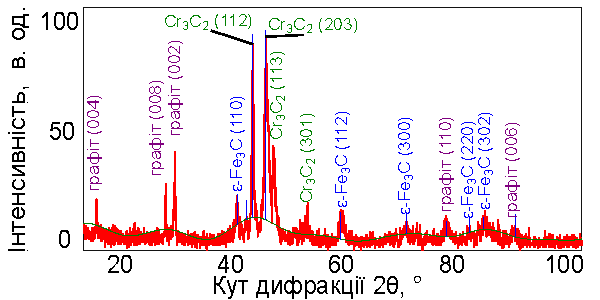
\includegraphics{pr_rigaku_peaks_Cr-W-C}
\end{figure}
\begin{alertblock}{Фазовий склад}
\centering
  $\epsilon\text{-}$F\textsubscript{3}C, Cr\textsubscript{3}C\textsubscript{2}, C(графіт)
\end{alertblock}
\end{frame}

\begin{frame}
\begin{figure}[H]
\centering
\caption{Дифрактограма зразка W-Cr-C}
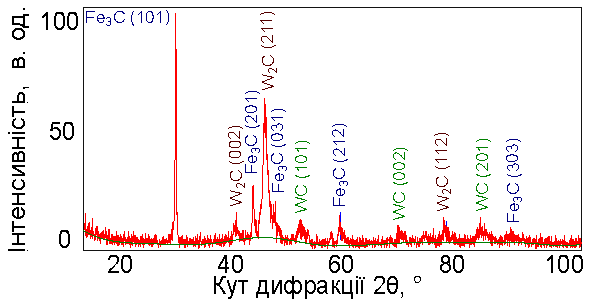
\includegraphics{pr_rigaku_peaks_W-Cr-C}
\end{figure}
\begin{alertblock}{Фазовий склад}
\centering
  WC, W\textsubscript{2}C, Fe\textsubscript{3}C
\end{alertblock}
\end{frame}

\begin{frame}
\begin{figure}[H]
\centering
\caption{Дифрактограма зразка W-C-Cr}
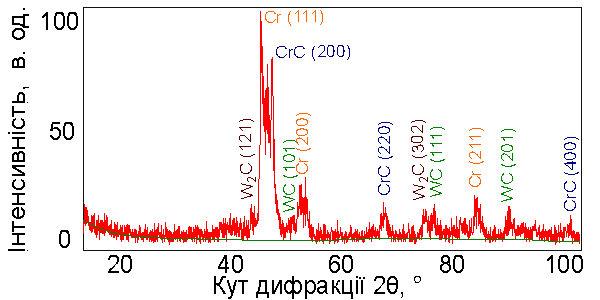
\includegraphics{pr_rigaku_peaks_W-C-Cr}
\end{figure}
\begin{alertblock}{Фазовий склад}
\centering
Cr, W\textsubscript{2}C, WC, СrC
\end{alertblock}
\end{frame}

\begin{frame}
  \begin{figure}[H]
  \centering
  \caption{Дифрактограма зразка C-Cr-W}
  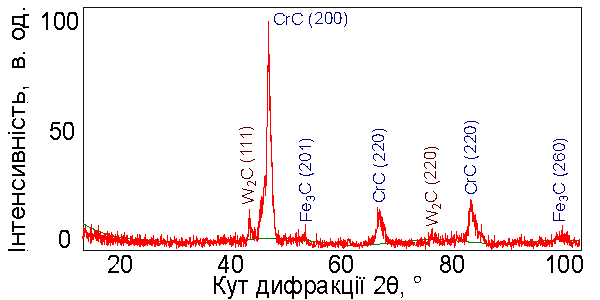
\includegraphics{pr_rigaku_peaks_C-Cr-W}
  \end{figure}
  \begin{alertblock}{Фазовий склад}
  \centering
Fe\textsubscript{3}C, CrC, W\textsubscript{2}C
  \end{alertblock}
\end{frame}


\section{Мікродюрометричний аналіз}

\begin{frame}
\begin{figure} % TODO АНАЛОГІЧНО ГРАВІМЕТРИЧНОМУ
  %\caption{Мікротвердість та мікроструктура (W-Cr-C)}
  \begin{minipage}[c]{0.49\textwidth}
    \includegraphics[width=\linewidth]{plt_pr_hard_C-Cr-W.pdf}\\[2mm]
    \includegraphics[width=\linewidth]{plt_pr_hard_Cr-W-C.pdf}
  \end{minipage}%
  \hfill
  \begin{minipage}[c]{0.49\textwidth}
    ~
    \includegraphics[width=\linewidth]{plt_pr_hard_W-C-Cr.pdf}\\[2mm]
    \includegraphics[width=\linewidth]{plt_pr_hard_W-Cr-C.pdf}
  \end{minipage}
\end{figure}
\end{frame}


\section{Випробування на зносостійкість}
\begin{frame}
\begin{figure}
  %\caption{Мікротвердість та мікроструктура (W-Cr-C)}
  \begin{minipage}[c]{0.49\textwidth}
    \includegraphics[width=\linewidth]{plt_pr_wear_C-Cr-W.pdf}\\[2mm]
    \includegraphics[width=\linewidth]{plt_pr_wear_Cr-W-C.pdf}
  \end{minipage}%
  \hfill
  \begin{minipage}[c]{0.49\textwidth}
    \includegraphics[width=\linewidth]{plt_pr_wear_W-C-Cr.pdf}\\[2mm]
    \includegraphics[width=\linewidth]{plt_pr_wear_W-Cr-C.pdf}
  \end{minipage}
\end{figure}
\end{frame}

\section{Порівняння отриманих властивостей}
\begin{frame}
\begin{figure}[H]
\centering
\caption{Порівняння максимальної мікротвердості та зносостійкості}
\label{fig:comp_wh}
\includegraphics[width=0.9\textwidth]{pr_comp_wh.pdf}
\end{figure}
\end{frame}


\section{ВИСНОВКИ}

\begin{frame}
\small
\vspace{-0.2cm}
\begin{exampleblock}{Встановлено можливість створення}
 функціональних покриттів товщиною 15-30~мкм на поверхні сталі~45 в процесі пошарового ЕІЛ W-, Cr-, C-анодами.
\end{exampleblock}

\begin{alertblock}{Встановлено підвищення поверхневої мікротвердості}
 сталі~45 від 11,5 ГПа до 18,9~ГПа після нанесення електроіскрових покриттів за всіма запропонованими схемами за рахунок наявності твердих розчинів матеріалів електродів та карбідів WC, W\textsubscript{2}C, Fe\textsubscript{3}C, Cr\textsubscript{3}C\textsubscript{2}, CrC.
\end{alertblock}

\begin{alertblock}{Виявлено, що зносостійкість покриттів}
зростає в ряду C-Cr-W~$\rightarrow$~W-C-Cr~$\rightarrow$~W-Cr-C~$\rightarrow$~Cr-W-C у 2,9-23~рази у порівнянні з необробленою поверхнею сталі~45.

Найвищу зносостійкість має покриття Cr-W-C за рахунок наявності вільного графіту.

\end{alertblock}
\end{frame}

\end{document}
